Nella sezione \emph{Stato Containers} l'utente può prendere visione dell'elenco dei container sulla macchina e eseguire alcune operazioni su di essi.

\begin{figure}[H]
    \begin{center}
    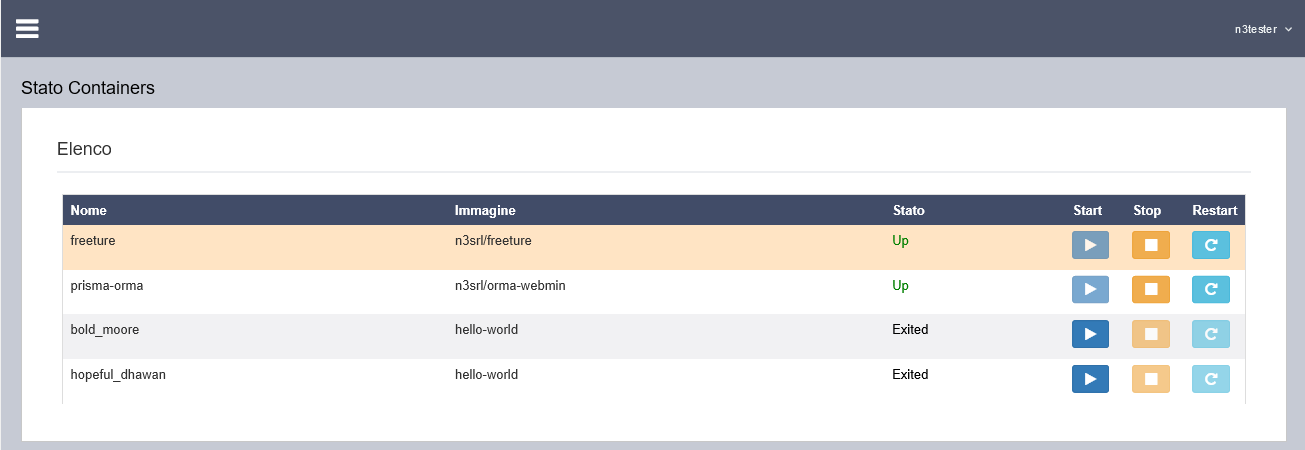
\includegraphics[width=\textwidth]{images/full-containers.png}
    \caption{Sezione \emph{Stato Containers}.}
    \end{center}
\end{figure}

\subsection{Visualizzazione container}

Nel dettaglio, i container sono organizzati in una tabella, realizzata con DataTables. Per ciascuno è riportato \textbf{nome del container}, \textbf{nome dell'immagine} e \textbf{stato corrente}. Gli stati possibili di un container sono:
\begin{itemize}[noitemsep,nolistsep]
    \item \emph{Up}: il container è attivo;
    \item \emph{Restarting}: il container si sta riavviando;
    \item \emph{Exited}: il container non è attivo.
\end{itemize}

\subsection{Avvio, riavvio e interruzione container}

L'utente ha la facoltà di interagire con i container elencati con tre pulsanti disponibili che consentono di:
\begin{itemize}[noitemsep,nolistsep]
    \item Avviare il container (\textbf{Start}), possibile solo se un container è fermo;
    \item Riavviare il container (\textbf{Restart}), possibile solo se un container è attivo o si sta riavviando;
    \item Fermare il container (\textbf{Stop}), possibile solo se un container è attivo o si sta riavviando.
\end{itemize}

I pulsanti inerenti a operazioni non possibili in quel momento risultano disattivati all'utente.

Il server per realizzare le richieste dell'utente deve prima accedere in SSH all'host dei container e solo successivamente eseguire i comandi Docker.